\section{Background} \label{background}

REs involving relations have received increasing attention recently;
especially in the context of spatial referring expressions in situated
generation (e.g., \cite{kelleher06:_increm_gener_of_spatial_refer}),
where it is particularly natural to use expressions involving spatial
relations such as ``the ball on top of the cube.''  However, the
classical algorithm
by~\shortcite{dale91:_gener_refer_expres_invol_relat} was shown to be
unable to generate satisfying REs in practice (see the analysis over
the \emph{cabinet corpus}
in~\cite{viethen06:_algor_for_gener_refer_expres}).  Furthermore, the
Dale and Haddock algorithm and many of its successors (such
as~\cite{kelleher06:_increm_gener_of_spatial_refer}) are vulnerable to
the problem of \emph{infinite regress}, where the algorithm enters an
infinite loop, jumping back and forth between descriptions for two
related individuals, as in ``the book on the table which supports a
book on the table \ldots''

\shortcite{arec2:2008:Areces,arec:usin11} have proposed low complexity
algorithms for the generation of relational REs
%(including references to sets) 
that eliminate the risk of infinite regression.  These algorithms are
based on variations of the partition refinement algorithms
of~\shortcite{paig:thre87}.  The information provided by a given scene
is interpreted as a relational model whose objects are classified into
sets that fit the same description.  This classification is
successively \emph{refined} till the target is the only element
fitting the description of its class.  The existence of an RE depends
on the information available in the input scene, and on the expressive
power of the formal language used to describe elements of the
different classes in the refinement.

Refinement
algorithms %presented in~\cite{arec2:2008:Areces,arec:usin11}
effectively compute REs for all individuals in the domain, at the same
time. The algorithms always terminate returning a formula of the
formal language chosen that uniquely describes the target (if the
formal language is expressive enough to identify the target in the
input model).
%\shortcite{arec2:2008:Areces}
%show that the refinement algorithm using the description language \el  is capable of generating 67\% of 
%the relational REs in the~\cite{viethen06:_algor_for_gener_refer_expres} dataset, when all possible orders of the relations in the domain are considered. This is in sharp contrast with the analysis 
%done in~\cite{viethen06:_algor_for_gener_refer_expres} over the cabinet corpus, of algorithms based in Dale and Reiter's original proposal.    


Refinement algorithms for GRE are based on the following basic idea:
given a scene $S$, the objects appearing in $S$ are successively
classified according to their properties into finer and finer
classes. A description (in some formal language $\mathcal{L}$) of each
class is computed every time a class is refined. The procedure always
stops when the set of classes stabilizes, i.e., no further refinement
is possible with the information available in the scene\footnote{Of
  course, if we are only interested in a referring expression for a
  given target we can stop the procedure as soon as the target is the
  only element of some of the classes.}.  If the target element is in
a singleton class, then the formal description of that class is a
referring expression; otherwise the target cannot be unequivocally
described (in $\mathcal{L}$).

It is clear that a scene can be encoded in different ways as a
relational model (for example in \ref{figure22}, we could argue that
$e_1$ is also \emph{leftof} $e_2$, not considered because they are no
touching). The algorithm assumes that these issues have been resolved
and that the model encodes a suitable representation of the scene we
want to describe.  Moreover, we will assume that all relations are
\emph{binary}.  We will not consider relations of arity greater than
two (relations of higher arity can be encoded as binary relations via
reification, if necessary).

On termination, the algorithm computes what are called the
$\mathcal{L}$-similarity classes of the input model $\gM$.
%Intuitively, the referring expression ``\textsf{ball}'' and ``\textsf{cube}''  are more specific and then contain more information than $\top$.

%There is many $\mathcal{L}$, we will name $\alc$ and $\el$

%ACA VOY A PONER gramatica para generar... ALC y EL no quedaria bien aca, hay que ver lo agregamos antes o no hace falta
In what follows, we use formulas of the $\el$ description logic
language~\cite{baad:desc03} to describe refinement classes
\footnote{Notice, though, that the particular formal language used is
  independent of the main algorithm, and different
  add$_{\mathcal{L}}$($\varphi$,\RE) functions can be used depending
  on the language involved.}.  As discussed
in~\cite{arec2:2008:Areces}, this language is suitable for describing
conjunctive and relational REs, which are the ones we find in corpora.

 The input to the algorithm will be a relational model $\mathcal{M} =
 \tup{\Delta, \interp{\cdot}}$, where $\Delta$ is the non-empty domain
 of objects in the scene, and $\interp{\cdot}$ is an interpretation
 function that assigns to all properties in the scene their intended
 extension.  For example, the scene shown in Figure~\ref{figure22}
 could be represented by the model $\gM=\tup{\Delta,\interp{\cdot}}$
 shown in Figure~\ref{GRE3D7-stimulus-graph}; where $\Delta =
 \{e_1,\ldots,e_7\}$, and $\interp{\textsf{red}}$ is $\{e_2, e_4, e_5,
 e_7\}$.

$\top$ is a formula that represents the most general description whose
interpretation includes all elements of the model. It could be realize
as the RE with the noun ``\textsf{thing}''. We say that a formula is
\emph{subsumed} by other formulas, if it extension can be cover by the
union of the extensions of the other formulas. For example, in
Figure~\ref{figure22}, $\top$ is subsumed by ``\textsf{ball}'' and
``\textsf{cube}'', because $\interp{\top}$ = $\interp{\textsf{ball}}
\cup \interp{\textsf{cube}}$.
%= $\{e_2, e_4, e_6, e_7\}$, it is $\{e_1, e_2, e_3, e_4, e_5, e_6, e_7\}$ = $\{e_1, e_3, e_5\} \cup \{e_2, e_4, e_6, e_7\}$. 
Intuitively the formula ``\textsf{cube}'' or ``\textsf{ball}'' have more information than $\top$, for each element of $\top$, there is a formula that gives more information, say ``\textsf{cube}'' is more informative than say ``\textsf{thing}''.\\

In the following we will explain an example of execusion of the
algorithm shown in Figure~\ref{algoritmoOriginal} taking into account
the $\el$ logic language. This algorithm where first presented
in~\cite{arec2:2008:Areces}.

\begin{figure}[h!]
\begin{center}
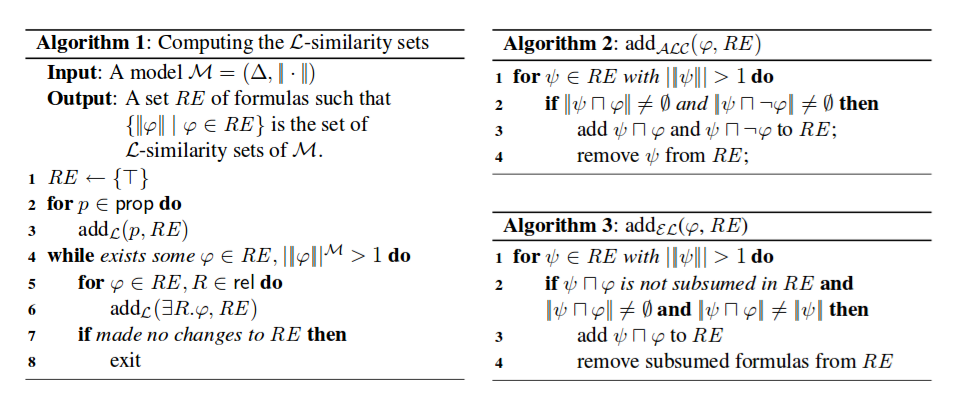
\includegraphics[width=\textwidth]{images/algoritmoOriginal.png}
\end{center}
\vspace*{-2em}
\caption{Algorithms for GRE with Description Logic}
\label{algoritmoOriginal}
\end{figure}

\subsection{An example of execution}

We will run the algorithm for the Scene~\ref{figure22}, the algorithm
start with a fixed list of properties and relations, suppose that
those lists are the following:

ordered properties (prop): \textsf{ball}, \textsf{cube}, \textsf{red}, \textsf{yellow}, \textsf{small}, \textsf{large}.\\
ordered relations (rel): \textsf{leftof}, \textsf{rightof}, \textsf{ontopof}, \textsf{bellowof}.

\begin{figure}
\begin{center}	
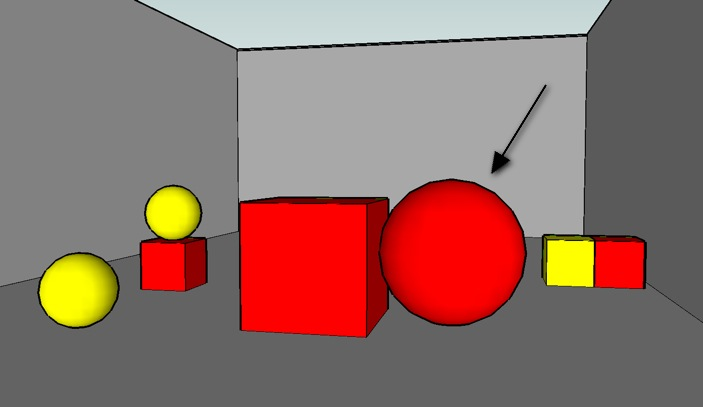
\includegraphics[width=.5\textwidth]{images/22.jpg}
\end{center}
\vspace*{-1.5em}
\caption{A 3D scene of geometric figures}\label{figure22}
\end{figure}

\begin{figure}
\begin{minipage}[b]{0.6\linewidth}
\centering
\begin{tikzpicture}
  [
    n/.style={circle,fill,draw,inner sep=3pt,node distance=1.4cm},
    aArrow/.style={->, >=stealth, semithick, shorten <= 2pt, shorten >= 2pt},
  ]
 \node[n,label=above:$e_1$,label=below:{
    \relsize{-1}$\begin{array}{c}
      \nLeft\\[-2pt]
      \nSmall\\[-2pt] 
      \nYellow \\[-2pt] 
      \nBall\end{array}$}] (a) {};

 \node[n,label=above:$e_2$,label=below:{
    \relsize{-1}$\begin{array}{c}
      \nLeft\\[-2pt]
      \nSmall\\[-2pt] 
      \nRed\\[-2pt] 
      \nCube\end{array}$}, right of=a] (b) {};

 \node[n,label=below:$e_3$,label=above:{
    \relsize{-1}$\begin{array}{c}
      \nTop\\[-2pt]
      \nLeft\\[-2pt]
      \nSmall\\[-2pt] 
      \nYellow\\[-2pt] 
      \nBall\end{array}$}, above of=b] (c) {};

 \node[n,label=above:$e_4$,label=below:{
    \relsize{-1}$\begin{array}{c}
      \nBig\\[-2pt] 
      \nRed\\[-2pt] 
      \nCube\end{array}$}, right of=b] (d) {};

 \node[n,label=above:$e_5$,label=below:{
    \relsize{-1}$\begin{array}{c}
      \nBig\\[-2pt] 
      \nRed\\[-2pt] 
      \nBall\end{array}$}, right of=d] (e) {};

 \node[n,label=above:$e_6$,label=below:{
    \relsize{-1}$\begin{array}{c}
      \nSmall\\[-2pt] 
      \nYellow\\[-2pt] 
      \nCube\end{array}$}, right of=e] (f) {};

 \node[n,label=above:$e_7$,label=below:{
    \relsize{-1}$\begin{array}{c}
      \nSmall\\[-2pt] 
      \nRed\\[-2pt] 
      \nCube\end{array}$}, right of=f] (g) {};

 \draw [aArrow,bend right=90] (b) to node[auto,swap]{\relsize{-1}$\nBelow$} (c);
 \draw [aArrow,bend right=90] (c) to node[auto,swap]{\relsize{-1}$\nOntop$} (b);

 \draw [aArrow,bend right=30] (d) to node[auto,swap]{\relsize{-1}$\nLeftof$} (e);
 \draw [aArrow,bend right=30] (e) to node[auto,swap]{\relsize{-1}$\nRightof$} (d);

 \draw [aArrow,bend right=30] (f) to node[auto,swap]{\relsize{-1}$\nLeftof$} (g);
 \draw [aArrow,bend right=30] (g) to node[auto,swap]{\relsize{-1}$\nRightof$} (f);

 \draw[dotted] (-.4,-1.7) rectangle (7.5,3.3);

 \end{tikzpicture}
\caption{Scene as a relational model}\label{GRE3D7-stimulus-graph}
\end{minipage}
\end{figure}


The algorithm always ends, and return RE, a set of formulas that describes each element in the domain (if that formula exists).\\

In the begining RE=$\{\top\}$ and its $\interp{\top}$ = $\{e_1, e_2, e_3, e_4, e_5, e_6, e_7\}$\\

The first loop for of the algorithm is in the properties. For each property realize add$_\el$ ($\varphi$, RE),

A formula $\varphi$ will be added to RE if its interpretation has at least one element, then for each formula $\psi$ in RE the conjunction 
$\varphi  \wedge \psi$ need to be not subsumed in RE, the $\interp{\varphi \cup \psi}$ need to be not empty, and its interpretation need to be distinct of $\interp{\psi}$. Then the subsumed formulas will be clean.

The first property is \textsf{ball}, RE = \{$\top$, \textsf{ball}\}, then the following property is \textsf{cube}, RE = \{$\top$, \textsf{ball}, \textsf{cube}\}, but now the $\interp{\textsf{ball}}$ = $\{e_1, e_3, e_5\}$, $\interp{\textsf{cube}}$ = $\{e_2, e_4, e_6, e_7\}$, so, we can delete $\top$, because it is subsumed to the two other formulas. The turn is now for the property \textsf{red}, $\interp{\textsf{red}}$ is: $\{e_2, e_4, e_5, e_7\}$, doing the intersection with the $\interp{.}$ of each formula in RE we obtain, $\{e_5\}$ and $\{e_2, e_4, e_7\}$, RE = $\{\textsf{ball}, \textsf{cube}, \textsf{ball} \wedge \textsf{red}, \textsf{cube} \wedge \textsf{red}\}$, following with \textsf{yellow}, we have, $\interp{\textsf{yellow}}$ = $\{e_1, e_3, e_6\}$ and we obtain RE = $\{\textsf{ball} \wedge \textsf{yellow}, \textsf{cube} \wedge \textsf{yellow}, \textsf{ball} \wedge \textsf{red}, \textsf{cube} \wedge \textsf{red}\}$. Note than here we already delete the formula \textsf{ball} because it was subsumed, and the formula \textsf{cube} too.
Doing the same with \textsf{small} we have RE = $\{\textsf{ball} \wedge \textsf{yellow} \wedge \textsf{small}, \textsf{cube} \wedge \textsf{yellow} \wedge \textsf{small}, \textsf{ball} \wedge \textsf{red}, \textsf{cube} \wedge \textsf{red}, \textsf{cube} \wedge \textsf{red} \wedge \textsf{small}\}$. Next property is \textsf{large} so, we have RE = $\{\textsf{ball} \wedge \textsf{yellow} \wedge \textsf{small}, \textsf{cube} \wedge \textsf{yellow} \wedge \textsf{small}, \textsf{ball} \wedge \textsf{red}, \textsf{cube} \wedge \textsf{red} \wedge \textsf{large}, \textsf{cube} \wedge \textsf{red} \wedge \textsf{small}\}$. Note that here we cannot add \textsf{large} to a formula $\textsf{red} \wedge \textsf{cube}$ because its interpretation has only one element, and the condition say that it need to have more than one.

Until now RE = $\{\textsf{ball} \wedge \textsf{yellow} \wedge \textsf{small}, \textsf{cube} \wedge \textsf{yellow} \wedge \textsf{small}, \textsf{ball} \wedge \textsf{red}, \textsf{cube} \wedge \textsf{red} \wedge \textsf{large}, \textsf{cube} \wedge \textsf{red} \wedge \textsf{small}\}$ and we have the following extensions: $\{e_1, e_3\}, \{e_6\}, \{e_5\}, \{e_4\}, \{e_2, e_7\}$ respectively. There is two formulas that can be refined more, the  $\textsf{ball} \wedge \textsf{yellow} \wedge \textsf{small}$ and $\textsf{cube} \wedge \textsf{red} \wedge \textsf{small}$ because they have more than one element each, so we enter en in the while cicle of Algorithm 1, in line 4. Now is the turn of relations, the first one is \textsf{leftof}, for each formula $\varphi$ in RE will try to add$_\el$ ($\exists \textsf{leftof}.\varphi$, RE). Note that $\psi$ only can be $\textsf{ball} \wedge \textsf{yellow} \wedge \textsf{small}$ or $\textsf{cube} \wedge \textsf{red} \wedge \textsf{small}$ because those are the ones that its interpretation have more than one element. There is not $\varphi$ and $\psi$ that can be apply. Continuing with \textsf{rightof} we add $\textsf{cube} \wedge \textsf{yellow} \wedge \textsf{small} \wedge \exists \textsf{rightof}. \textsf{cube} \wedge \textsf{red} \wedge \textsf{small}$, and so on with \textsf{topof} we add $\textsf{small} \wedge \textsf{red} \wedge \textsf{cube} \wedge \exists \textsf{ontop}. \textsf{small} \wedge \textsf{yellow} \wedge \textsf{ball}$ and the algorithm ends with RE = $\{\textsf{ball} \wedge \textsf{yellow} \wedge \textsf{small}, \textsf{cube} \wedge \textsf{yellow} \wedge \textsf{small}, \textsf{ball} \wedge \textsf{red}, \textsf{cube} \wedge \textsf{red} \wedge \textsf{large}, \textsf{cube} \wedge \textsf{red} \wedge \textsf{small}, \textsf{cube} \wedge \textsf{yellow} \wedge \textsf{small} \wedge \exists \textsf{rightof}. \textsf{cube} \wedge \textsf{red} \wedge \textsf{small}, \textsf{small} \wedge \textsf{red} \wedge \textsf{cube} \wedge \exists \textsf{ontop}. \textsf{small} \wedge \textsf{yellow} \wedge \textsf{ball}\}$, here all elements are in a singleton class and not further refinement can be done.


%can be applied to $cube \wedge red \wedge small$ but there is no formula which interpretation has more than one element to be apply with this one. The same happen for the other relations, so the algorithm ends.
%its interpretation is $\{e_7\}$ with $\psi$ is $cube \wedge yellow \wedge small$, the others combinations can't be apply because they don't do true the preconditions. The following relation is rightof, 

%leftof, rightof, ontopof, bellowof

%At this point we already have the target in a singleton set. So the formula for it is ``red and ball'', and also for s6 which formula is ``yellow cube''.\\
%As we show this algorithm depends of the order of properties and relations.\\


